%\documentclass{acm_proc_article-sp}
\documentclass[letterpaper]{article}
\usepackage{aaai}

\usepackage{times}
\usepackage{helvet}
\usepackage{courier}
\usepackage{url}
\usepackage{dsfont}
\usepackage{subfigure}
\usepackage{graphicx}
\usepackage{xspace}
\usepackage{multirow}
\usepackage{booktabs}
\usepackage{enumitem}
\usepackage{listings}
\usepackage{siunitx}
\usepackage{balance}
\usepackage{lastpage}
\usepackage[usenames,svgnames]{xcolor}
\usepackage{amsmath,array,graphicx}
\usepackage{kantlipsum}
\usepackage{appendix}
\usepackage{lipsum}
\usepackage{sidecap}
\usepackage{sparklines}
\usepackage{pgfplots}
\usepackage{tikz}
\usepackage[font=small,labelfont=bf]{caption}
\newcommand{\rs}[1]{\textcolor{ForestGreen}{RM: #1}}
\newcommand{\rp}[1]{\textcolor{Magenta}{RP: #1}}
\newcommand{\pcm}[1]{\textcolor{Red}{PCM: #1}}
\newcommand{\jp}[1]{\textcolor{Blue}{JP: #1}}
\renewcommand{\baselinestretch}{1.0}
\setlength{\emergencystretch}{50pt}
\setcounter{secnumdepth}{2}
\renewcommand{\sparklineheight}{2} 
\renewcommand{\sparklinethickness}{0.5pt}
\renewcommand{\sparkspikewidth}{1.2pt} 
\definecolor{sparkspikecolor}{named}{cyan}
\definecolor{sparklinecolor}{named}{black}

\begin{document}

%\permission{Permission to make digital or hard copies of all or part of this work for personal or classroom use is granted without fee provided that copies are not made or distributed for profit or commercial advantage and that copies bear this notice and the full citation on the first page. To copy otherwise, to republish, to post on servers or to redistribute to lists, requires prior specific permission and/or a fee.}
%\conferenceinfo{WWW Montreal, Canada}{'16}
%\copyright{Copyright 2015 ACM X-XXXXX-XX-X/XX/XX ...\$15.00.}

%\title{Large-scale analysis of social media campaigns on climate change}
\title{Please Sign to Save ... : When Petitions on Environmental Causes Succeed}

%or \title{Sign and Save... : How Online Petitions Succeed}
% "Petitions on Environmental Causes" is not really a term according to Google


\newcommand{\etal}[1]{#1~\emph{et al.}}

%\numberofauthors{5} %  in this sample file, there are a *total*
% of EIGHT authors. SIX appear on the 'first-page' (for formatting
% reasons) and the remaining two appear in the \additionalauthors section.
%
%\author{
% You can go ahead and credit any number of authors here,
% e.g. one 'row of three' or two rows (consisting of one row of three
% and a second row of one, two or three).
%
% The command \alignauthor (no curly braces needed) should
% precede each author name, affiliation/snail-mail address and
% e-mail address. Additionally, tag each line of
% affiliation/address with \affaddr, and tag the
% e-mail address with \email.
%
 % 1st. author
% \alignauthor Julia Proskurnia \\
%        \affaddr{\'{E}cole Polytechnique F\'{e}d\'{e}rale de Lausanne}\\
%        \affaddr{Lausanne---Switzerland}\\
%        \email{iuliia.proskurnia@epfl.ch}
% 2nd. author
% \alignauthor Karl Aberer\\
% 	     \affaddr{\'{E}cole Polytechnique F\'{e}d\'{e}rale de Lausanne}\\
%        \affaddr{Lausanne---Switzerland}\\
%        \email{karl.aberer@epfl.ch}
% 3rd. author
% \alignauthor Philippe Cudr\'{e}-Mauroux\\
% 	    \affaddr{University of Fribourg}\\
%        \affaddr{Fribourg---Switzerland}\\
%        \email{phil@exascale.info}

\maketitle


\begin{abstract}

% Climate change
Social media have become one of the key platforms to support the debate on climate change.
% Campaigns and e-petitioning
In particular, Twitter allows easy information dissemination when running environmental campaigns.
Yet, the dynamics of these campaigns on social platforms still remain largely unexplored.
% Role of the petitions in the environmental campaigns
In this paper, we study the success factors enabling online petitions to attain their required number of signatures.
% Petition success based on the campaign or Twitter activity
We present an analysis of e-petitions and identify how their number of users, tweets and retweets correlate with their success. In addition, we discuss how campaigns with high user engagement are the most active in promoting petitions on Twitter \pcm{I don't understand that}.
% Findings...
Finally, we present an annotated corpus of petitions posted by environmental campaigns together with their corresponding tweets \pcm{why? towards what goal? seems disconnected to the res}.

\end{abstract}

 % A category with the (minimum) three required fields
% \category{H.3.1}{Information Storage and Retrieval}{Content Analysis and Indexing}
 %A category including the fourth, optional field follows...
% \category{J.4}{Social and Behavioral Sciences}{Sociology}
% \terms{Algorithms, Experimentation}
%\keywords{public campaign analysis, action extraction, time series analysis}

\vspace{1em}

\setlength{\parskip}{0pt} % 1ex plus 0.5ex minus 0.2ex}
\setlength{\parindent}{0pt}

%!TEX root = ../sig-alternate.tex
\section{Introduction}
\label{sec:intro}

% Context: 
% Environment and wildlife issues are linked to the human-induced climate change~\cite{solomon2009irreversible} and therefore, humanity is concerned about the ways to improve the situation.
%
% As a result, public campaigns have became one of the major instruments to increase awareness and mobilize people towards issues of climate change and animal welfare~\cite{Pearce2014}.
%
% In turn, public campaigns often leverage e-petitioning~\cite{mosca2009petitioning} to reach out to local, national governments or institutions.
% Outcome of the petitions is relatively easy to extract, since such information is usually provided by petition aggregator web cites. This information can help quantify the performance of the public campaigns and petitions themselves, i.e., by a successful petition we understand a petition that has reached specified number of signatures.

The discourse on climate change is often focused on the impact it has on the environment and on  wildlife~\citeauthor{solomon2009irreversible} \shortcite{solomon2009irreversible}.
To bring these issues in the public spotlight, social media campaigns have proved to be an effective instrument to raise awareness and mobilize masses~\citeauthor{Pearce2014} \shortcite{solomon2009irreversible}.
To further push for concrete actions from governments or public entities, many campaigns resort to e-petitioning~\citeauthor{mosca2009petitioning} \shortcite{solomon2009irreversible}, whose success is also much easier to assess: reaching or not a required number of signatures.
Information about the number of signatures obtained for a given e-petition is often publicly available via e-petitions aggregators websites such as \url{thepetitionsite.com}, \url{avaaz.org}, \url{change.org} etc., and can be used as a proxy for the performance of the public campaigns and petitions themselves.

% Existing opportunity
%
% 1.
% E-petitions share many features and qualities with other social platforms, e.g., can create and share content.
% Since Twitter remains one of the easiest way to disseminate information on the Web to a large groups of people, we analyse tweets mentioning petitions posted with the environmental campaign hashtags on Twitter.
% It is important for the campaign leaders to know how petitions are promoted by other campaigns on Twitter and if a petition success is caused by any of the Twitter platform aspects (users that tweet the petitions, petitions tweets outside of the campaign, type of campaign, final goal of the petitions etc.)

% Our goal
%   Research questions and major findings:
In this work, we tackle two main research questions.

\textbf{RQ1:} \textit{Which types of the public campaigns use petitions in their agenda?}
% What is the role of petitions in various types of environmental campaigns?}
To answer this question, we study several environmental campaigns than were run in the beginning of 2015, measuring the incidence of e-petitioning as an instrument for campaigning across different types of campaigns (awareness, mobilization). We find that petitioning is particularly important during mobilization campaigns.\footnote{Mobilization campaigns refer to the campaigns whose primary goal is to engage and motivate a wide range of partners, allies and individual at the national and local levels, towards a particular problem or issue. While awareness campaigns refer to the campaigns whose primary goal is to raise people’s awareness regarding a particular subject, issue, or situation.}

\textbf{RQ2:} \textit{What makes a petition promoted by a public campaign successful?} We answer this question by making a feature analysis and comparing tweets that belong to public campaigns to individual tweets. 
%
We propose a set of social and contextual features and show how the required number of signatures for an environmental petition is  correlated to its outcome.
Additionally, we release an annotated corpus with the petitions, their tweets and outcomes\footnote{https://github.com/toluolll/PetitionsDataRelease}.
For this study we focus on Twitter, which remains one of the main channels for social media campaigns, also providing relatively easy access to campaign data.

% Related work and our position/contributions x 2 paragraphs
% Campaigns/Protests on Climate Change
\textbf{Climate Change Discourse on Social Media.} Climate change is a highly discussed topic. \citeauthor{Kirilenko2014} \shortcite{Kirilenko2014} overview the climate change domain, its polarization, discussion over time etc. \citeauthor{Olteanu2015} \shortcite{Olteanu2015} study how various climate related events are highlights by various media sources.
Variety of public campaigns use social platforms to increase awareness or mobilize people~\citeauthor{Mahmud2014} \shortcite{Mahmud2014}.
\citeauthor{Tufekci2013} \shortcite{Tufekci2013} describes how the on-line attention can be driven towards particular politicized persona, while \citeauthor{gonzalez2013networked} \shortcite{gonzalez2013networked} analyse information transmission during protests.
\citeauthor{hestres2013preaching} \shortcite{hestres2013preaching} studies public mobilization and online-to-offline social movement strategies for two major environmental movements. Unlike the prior work, we analyze a over 100 environmental campaigns as well as their effect on the petition success.
% TODO: Possible add to the previous section one of the findings we will have!!!

% Petitions
\textbf{Characterizing E-petitions.} Various works were conducted to analysis the e-petitions on various petition aggregators.
\citeauthor{Hale2013} \shortcite{hestres2013preaching} describe a temporal analysis of 8K petition on the UK No. 10 Downing Street and make an observation towards early signs of successful petition (large number of signatures during the first days).
\citeauthor{Huang2015} \shortcite{Huang2015} analyse ``power'' users that produce petitions. The authors have shown that only 1\% of general topic petitions on \url{change.org} reaches their goal.
However, to the best of our knowledge, we are the first to analyze which factors predict the success of an environmental petition based on the internal and external attributes of the corresponding public campaign on Twitter.
% Kickstarter
On the other hand, analysis of the e-petitions can be compared to the crowdfunding, since in both fields desired and obtained support can be analysed.
\citeauthor{Etter2013} \shortcite{Etter2013} study various prediction techniques for Kickstarter campaigns.
Later, \citeauthor{An2014} \shortcite{An2014} analyse investor activity on Kickstarter and make recommendations of projects based on their activity on Twitter. Unlike aforementioned works, we focus on the climate change and animal welfare petitions, as a part of the environmental public campaigns on Twitter.


% Implications/Impact etc...
In this work, we found that 25\% of the petition posted with environmental campaigns hashtags on Twitter obtained their required number of signatures.
Moreover, we identify a number of features that can act as indicators for the success of the petitions.
This information might be of a great interest to the environmental activists and campaign leaders as it can influence the success of the message they are conveying to the public.
It should be noted that the techniques presented below are not restricted to the environmental domain and could be applied to any related setting.

% Disclaimers
% In Section~\ref{sec:dataset}, we describe our dataset, its main characteristics, filtering and annotation we apply. We then present in Section~\ref{sec:petition_analysis} petitions' position within environmental campaigns and outside of then within Twitter platform. Finally, we highlight major finding (Section~\ref{sec:discussion}) and conclude in the end.
%!TEX root = ../sig-alternate.tex
\section{Data Collection, Cleansing and Insights}
\label{sec:dataset}

Our study is based on the collection of roughly 7,500 tweets and retweets belonging to 240 petitions related to campaigns on environmental causes, which were posted from January 2015 to April 2015. Specifically, we consider a tweet to be related to a given petition if it contains the word ``petition'' in its content. This filter is generic to capture mentions from the tweet text and URL itself while having small ambiguity.

\textbf{Campaigns dataset and petition tweets:}
% * Environmental campaigns on Twitter and their collection by means of power users and crowdsourcing.
In order to analyze \textbf{RQ1},
we have used an annotated corpus of such campaigns for a given period on Twitter\footnote{https://github.com/toluolll/CampaignsDataRelease}.
Our campaign corpus consists of 101 public environmental campaigns with over 850K unique tweets. 
We assume that each campaign has a uniquely identified hashtag, e.g., \#saveafricananimals, \#tweet4dolphins etc.
Moreover, all the campaign hashtags are labeled by (a) a high-level goal, e.g., awareness or mobilization type, and (b) a user engagement pattern over time, e.g., one-day campaigns, ever-growing, annual, inactive\footnote{
Ever-growing campaigns have constantly growing number of users posting with the hashtag.
One-day campaigns have the most user activity that happens primarily on the first mention of the hashtag.
Annual campaigns are mentioned annually, e.g., yearly, monthly. Inactive campaigns have very low user engagement overall.}.
These are the main categories that will be used in our analysis.
Among those, ``ever-growing'' campaigns are the most interesting ones since they have constantly growing number of people that are involved in their action on Twitter.

% * Elimination of duplicates and merge unobvious duplicates
We extracted all ``petition'' tweets from the annotated collection of environmental public campaigns tweets.
Here we present an example of a tweet with a petition URL: \textit{``.@thetimes Petiton: Call for Safer Storage of Nuclear Waste in over 80 USA cities. http://tiny.cc/okzicx  \#SaveFukuChildren''}.
Such tweets were identified in 39 (out of 101) campaigns. 15K tweets belonged to unique unresolved links (excluding tweets with broken links).
In addition, we resolved, stored and annotated all petition URLs. As a result, we found 294 unique petition links and 158 broken or outdated links.
For valid petition links, we have stored their resolved URL. We further used this information to eliminate URLs that point to the same petition.
This process has resulted in 240 unique petitions.

% * Limitation for further exploration                      
\textbf{Tweets with petitions:}
Regarding \textbf{RQ2},
it should be noted that the campaign tweets collection does not account for the overall distribution of the petition tweets across the whole Twitter. 
Therefore, we collected additional data as we describe below.
To minimize the bias in our collection, we further collected tweets that contain one of 240 petition via \url{backtweets.com}. For this task, we used the collection of the extracted URLs with their resolved links (if applicable) and requested \url{backtweets.com} to return all historical tweets that mention the given URL.
Clearly, this still results in only a subset of the petition tweets since it does not account for the URL redirects and shortening. However, we aim for a best effort collection, which gives us a clearer picture on the distribution of the petitions tweets.
As a result, we enriched the tweet collection with over 1,700 new tweets without campaign hashtag.

\textbf{Thepetitionsite.com.} To compare campaign petitions with other environmental petitions, we additionally collected all the environmental and animal welfare petitions from the major petition aggregator\footnote{Accessed on the 16th Feb 2016} \url{thepetitionsite.com} and corresponding tweets from \url{backtweets.com}. This resulted in over 2'800 petitions with the following properties: (a) 35\% of them are successful; (b) 79 of them are in the campaign dataset, (c) 186 of them are mentioned on Twitter with their direct URLs.

\textbf{Dataset preprocessing}
To be able to compare petitions with each other, we use both campaign and non-campaign tweets.
% TODO: Next sentence might be redundant...
A petition $p$ is characterized by its signature goal $S(p)$, collected signatures $C(p)$, $SignatureRate = \frac{C(p)}{S(p)}$ and the following set of Twitter related features $T_i(p)$:\\
\textit{(1)} Number of unique users posted the petition url; 
\textit{(2)} Number of tweets with url;
\textit{(3)} Number of followers of the users posting petition tweets with/without a campaign hashtag;
\textit{(4)} Number of tweets with campaign hashtags vs without.
%!TEX root = ../sig-alternate.tex
\section{Petition analysis}
\label{sec:petition_analysis}

Given the list of petitions corresponding to campaigns on environmental issues on Twitter (described above), we first present an analysis on the petitions usage within different types of public campaigns and then analyze petition success by its visibility on Twitter.
%Finally, we propose a model to classify success of a particular campaign petition on Twitter.

\subsection{Petitions and tweets stats}
% * Number with petitions tweet stats: number of tweets; number of urls; number of valid urls with petitions;
Table~\ref{tab:petition_tweets} includes the basic figures extracted from our list of petitions\footnote{Latest petition signatures reassessment was on 28 Jan 2016.}.
Surprisingly, we notice that failed petitions aimed to gather only about half as much signatures as successful campaigns.
Furthermore, in our data, about a quarter of the petitions were successful, as opposed to only 1\% as found by~\citeauthor{Huang2015} \shortcite{Huang2015} across a broader range of petitions.
Overall, the tweets corresponding to the successful petitions are more likely to be passed on, i.e., they are retweeted about 4 times more frequently.

After a deeper inspection of the petition collection, we identified that over 6\% of the petitions in our dataset have a low signature goal $S(p)$, i.e., under 1,000 required signatures, out of which 13\% are identified as successful (as they reach their goal).
On the other hand, around 50\% of the petitions have a high initial goal (over 30,000) among which 35\% are successful.
Additionally, we observed that 39 petitions reached over 100K signatures while 130 petitions collected over 10K signatures.
The distribution of collected signatures is shown in Figure~\ref{fig:signatures_vs_rank}; it follows a Zipf distribution.

\begin{table}[hbt!]
\centering
\begin{tabular}{lccc}
			& \textit{Successful} & \textit{Failed}	\\ \midrule
Petitions					& 61		& 179		\\
Original tweets				& 601		& 716		\\
Original tweets users 		& 245		& 313		\\
Retweets						& 4828		& 1451 		\\
Retweets users				& 3965		& 1207		\\
Median $S(p)$				& 50000		& 15000		\\
Median $C(p)$				& 62997		& 6226		\\
\multicolumn{3}{l}{\textit{Petition tweets without campaign hashtags}}	\\ \midrule
Tweets						& 1054		& 707		\\
Users 						& 626		& 472		\\
\end{tabular}
\caption{Global statistics of the petition dataset of environmental campaigns. We show the data for the successful and failed petitions, as well as total numbers. Users are unique individuals who tweeted the petition URLs at least once. $S(p)$ and $C(p)$\footnote{Standard deviation for both $S(p)$ and $C(p)$ is within 270K} for successful and failed petitions are highlighted in the table. Additionally, we show statistics of the petition tweets that do not have a campaign hashtag.}
\label{tab:petition_tweets}
\end{table}

\begin{figure}
\centering
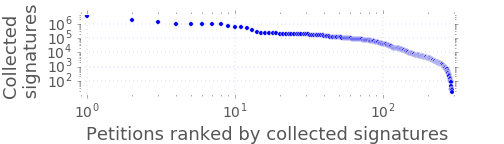
\includegraphics[width=\columnwidth]{figures/petitionsVSrank.png}
\caption{The final number of signatures received by each petition. The red line indicates the required number of signatures. A change in the slope of the zipf distribution occurs at 1K signatures, which represents a threshold for a petition to make a potential impact.}
\label{fig:signatures_vs_rank}
\end{figure}

\subsection{Petitions in public campaigns on Twitter}
% Information regarding environmental campaigns, types etc.
% Our findings:
% (a) only mobilization and single awareness; annual campaign with big number of msgs and failure rate.
% (b) doimated by the ever-growing campaigns.
% (c) Interesting examples (http://www.petitions.moveon.org/sign/legalize-hemp-farming/ - askdrh;
% https://you.38degrees.org.uk/petitions/stop-the-fracking-cover-up-by-defra - talkfracking (fracking censorship to delete.))

The following subsection provides answers for \textbf{RQ1} based on our analysis.
With only two exceptions, all the petitions were promoted through mobilization campaigns. The two exceptions are ``\#talkfracking'' and ``\#worldlovefordolphins'', which are both awareness campaigns.
Interestingly, these petitions with public campaigns hashtags were directed towards long-term plans, e.g., preventing ``covering up'' hydraulic fracturing by some organizations, or legalizing hemp farming.

As described in the Data Collection section, the campaign corpus is also annotated according to user engagement patterns for each campaign, and consists of four main types: one-day, ever-growing, annual, inactive.
We found that ``ever-growing'' campaigns (``\#saveafricananimals'', ``\#tweet4dolphins'' etc.) are the most active at tweeting about the petitions.
The rest $\sim$15\% of the campaigns are mainly ``inactive'' (``\#savethereef'', ``\#votegreen2015'').
Not surprisingly, ``one-day'' campaigns do not use petitions as their instruments given the very short timespans of such campaings.
Among campaigns with petitions, we also identified one ``annual'' campaign (``\#worldlovefordolphinsday'') that is advertising multiple ``Protect Dolphins'' petitions that tend to have a high failure rate.
Overall, there is no clear distinction between campaigns in terms of having dominantly successful petitions.
However, mobilization and ``ever-growing'' campaigns were the most active with petitions on Twitter.

\subsection{Campaign petitions on Twitter}
After data collection, cleaning and preprocessing, we extracted a number of features from the tweets containing a petition URL.
This process is explained in Section~\ref{sec:dataset} in detail.
To answer \textbf{RQ2}, we built a binary decision tree classifier\footnote{ http://scikit-learn.org } over our petition tweets collection using our set of features.

On average, the resulting tree has a relatively high branching factor, however a few paths are better at predicting the petition success.
We observe that the higher the signature goal, $S(p)$, of a particular petition, the more likely it is to succeed.
In particular, for the signature goal between between 100K and 300K 88\% of the petitions were successful.
However, setting a high petition goal may not guarantee its success. Success might also be correlated with various external factors, i.e., problem that a petition tries to address, external promotion (Facebook etc.), location of the petition owner etc.
Hence, the success factors for those campaigns are very different from the success factors of Kickstarter campaigns, for which failed campaigns have goals (amount of money) about three times higher than successful campaigns~\citeauthor{Etter2013} \shortcite{Etter2013}.

In our case, over 92\% of the petitions with $S(p)$ higher than 100K obtained their required number of signatures.
% TODO: Add some motivation, examples etc...
Regarding $T_3(p)$, the lower the average number of followers a campaign activist has, the less likely the petition is to attain the required number of signatures.
Similarly, the higher the average number of followers a user posting the petition URL without campaign hashtags has, the more likely the petition is to attain the required number of signatures.
We observe that the average number of followers is 10x higher for users outside of the campaign compared to campaign activists. 

\paragraph{Further Insights Towards RQ2}
Since it is not trivial to provide step-by-step instructions on how to drive your petition towards success in general, we would like to highlight some additional key points from our analysis.

% \pcm{I like the two following points; perhaps those should be the questions you pose in the introduction (research questions); then you could explicitly say that you come back to those questions here}

\textbf{Does petition success correlate with the number of tweets? - Yes.} We observed uniform distribution for the petitions with 0 tweets found on \textit{backtweets.com} in terms of $SignatureRate$. On the contrary, for the petitions with several tweets carrying its direct URL, $T_2(p)$, we observed a very high fraction of successful petitions (88\%). Pearson correlation for petitions with multiple tweets is 0.64 with \(p < 0.05\). This effect is particularly strong when we consider only retweets or tweets without campaign hashtags, $T_4(p)$. We observed similar behavior for \textit{thepetitionsite.com}.

\textbf{Does the number of users posting about the petition affect its success? - Yes.} We binned the petitions from the campaign corpus based on the $SignatureRate$, and extracted the average number of unique users posting about the petition in each bin. Figure~\ref{fig:signatures_vs_users} shows a boxer plot with the 25th, 50th and 75th percentiles for each bin. As a result, Pearson correlation is over 0.7 with \(p < 0.003\).

\begin{figure}
\centering
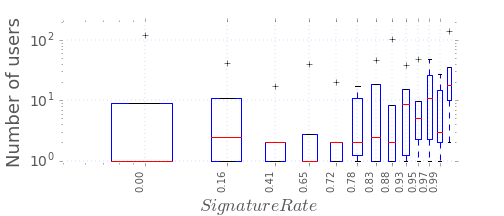
\includegraphics[width=\columnwidth]{figures/signaturesgoalVSnumusersCampaigns.png}
\caption{$SignatureRate$ against number of unique users posting about a petition on Twitter.}
\label{fig:signatures_vs_users}
\end{figure}

\textbf{Is it common to post (a) identical tweets without acknowledging original tweets or (b) retweet? - Retweet.} In our petition dataset we did not identify any duplicated tweets, i.e., tweets that are identical. Moreover, as shown in Table~\ref{tab:petition_tweets}, the number of retweets for the successful petitions is several times higher than the corresponding number for the unsuccessful ones.

\textbf{Which word features are more representative for tweets with successful petitions? - Uppercased.} We discovered that tweets with successful petitions have more words and uppercased words on average, by 9\% and 12\% respectively. We compared the distribution of the uppercased words between the collections of successful and failed petitions by computing the relative change for each word. We define it as follows: $RelativeChange = \frac{W_{succ} - W_{fail}}{W_{fail}}$, where $W_{succ}$ and $W_{succ}$ are the term frequencies of uppercased word $W$ for tweets with successful and failed petition. The top words from the successful collection are: ``ACTION'', ``URGENT'', ``WAZA'', ``PETITION'', ``SIGN'', while the unsuccessful petitions did not uppercase those words at all.

%!TEX root = ../sig-alternate.tex
\section{Conclusions}
% Conclusions and main results.
In this paper we introduce a dataset of environmental petitions that were promoted by major environmental public campaigns on Twitter.
We study the petition role as one of the actions performed by a public campaign.
We propose a model to identify successful petitions by their presence on Twitter and highlight the main aspects featuring a petition to obtain required number of signatures.
% We show that the more critical petition is, the more likely it is to have a high signature goal and the more likely it is to collect signatures.
Although, our dataset is limited in size, we made a best effort data collection and cleaning, and could observe the spread of the petitions within the public environmental campaigns and identify the major factors that may correlate with the success of the petition.
Our findings can provide helpful directions for all, leaders of the public campaigns, its participants, petition initiators and signers.

% Future work and limitation.
% 1.
Interesting future direction is to study the user aspect of the petition promoters on Twitter. In particular, we could identify the relations between petition signers and users who promote petitions on Twitter. The main difficulty here is to obtain this information for the large number of petition.

% 2.
Currently we propose a set of basic features and highlight the most valuable ones. The next step would be to explore time series properties of signatures, as well as, give actionable feedback on how to increase number of signers.

\bibliographystyle{aaai}
{
\begin{small}
\balance
\bibliography{sigproc}
\end{small}
}

\end{document}
